\begin{figure}[H]
    \centering

\begin{tikzpicture}
\pgfplotsset{
    every axis/.style={ymin=0},
    width=0.75\textwidth,
    height=0.25\textheight,
    xtick={1, 2, 3, 4, 5, 6, 7, 8},
    y axis style/.style={
    yticklabel style=#1,
    ylabel style=#1,
    y axis line style=#1,
    ytick style=#1}}
\begin{axis}[ scale only axis, xmin=1,xmax=8, axis y line*=left, xlabel=Number of Cores, ylabel=Execution time (s), y axis style=green!75!black]
    \addplot[smooth, green!75!black, mark=o, draw] 
    coordinates 
    {
        (1,944)
        (2,773)
        (3,734)
        (4,719)
        (5,700)
        (6,694)
        (7,698)
        (8,691)
    };
\end{axis}
%
\begin{axis}[ scale only axis, xmin=1,xmax=8, axis y line*=right, axis x line=none, ylabel=DEC (j), y axis style=blue]%
    \addplot[smooth, blue, mark=x] 
    coordinates 
    {
        (1,5140)
        (2,5425)
        (3,5571)
        (4,5575)
        (5,5600)
        (6,5661)
        (7,5615)
        (8,5523)
    };
\end{axis}
%
\begin{axis}[red, scale only axis, xmin=1,xmax=8, axis y line*=right, axis x line=none, ylabel=DEC per second (w)]%
\pgfplotsset{every outer y axis line/.style={xshift=2cm}, every tick/.style={xshift=2cm}, every y tick label/.style={xshift=2cm} }
    \addplot[smooth, red ,mark=+] 
    coordinates 
    {
        (1,5.372325)
        (2,6.956200)
        (3,7.57220)
        (4,7.75845)
        (5,7.992968)
        (6,8.15546)
        (7,8.06464)
        (8,8.04154494)
    };
\end{axis} 

\end{tikzpicture}
    \caption{The evolution of the DEC (blue), DEC per second (red) and execution time (green) as more cores are allocated to PCM on DUT 1}
    \label{fig:exp_3_dut_1_pcm_result}
\end{figure}